\chapter{Technische Grundlagen} \label{Technische_Grundlagen}

\section{Internet Protocol Version 4 (IPv4)} \label{ipv4}
\subsection{Allgemeines und Adressierungsschema}
Das Internet Protocol Version 4 ist im OSI-Modell auf Schicht 3 (Network-Layer) angesiedelt\cite{itu1994}. Es dient der \textit{Paketierung} von Daten und anschließenden Ende-zu-Ende-Vermittlung dieser \textit{Pakete} zwischen Netzwerk-Systemen. Dafür notwendig ist eine Adressierung: eine IPv4-Adresse besteht aus einer 32 Bit-Zahl, welche typischerweise dezimal dargestellt wird in so genannter \glqq dotted decimal\grqq{}-Schreibweise. Dafür wird die Binärzahl in vier Oktette mit einem Punkt aufgeteilt und die jeweiligen Oktette in dezimal umgerechnet.

{\centering 32 Bit Integer:\\
\textbf{00000001 0000001 000000011 00000100}\\
$\Downarrow$\\
\glqq Dotted Binary\grqq{}:\\
\textbf{00000001.00000010.00000011.00000100}\\
$\Downarrow$\\
Dotted Decimal (bekannte Schreibweise):\\
{\textbf{1.2.3.4}}\par}

Mit Hilfe von (Sub-)Netzmasken wird die Netzwerkgröße bestimmt. Ein Host mit der IP-Adresse 1.2.3.4 habe eine Netzmaske von 255.255.255.0. Diese Netzmaske entspricht in dotted binary:

{\centering\textbf{11111111.11111111.11111111.00000000}\par}

Die ersten 24 Bit sind für das Netzwerk reserviert (Network bits), die letzte 8 Bit sind Host bits. Dieses Netzwerk kann somit theoretisch aus $2^8 = 256$ Hosts bestehen, wobei die erste und letzte Adresse reserviert sind (Netzwerk- und Broadcast-Adresse).

Heutzutage üblich ist die so genannte Classless Inter-Domain Routing-Notation (CIDR), welche IP-Addresse und Netzmaske vereint. Wenn man die genannten Beispiele aus Adresse und Subnetzmaske zusammenführt, erhält man die IP-Adresse in CIDR-Notation: 1.2.3.4/24. /24 entspricht dabei den gesetzten Network bits.

Mit Hilfe der IP-Adresse und Netzmaske lässt sich ermitteln, ob sich ein anderer Host im gleichen \textit{Subnetz} befindet. Dafür berechnet das Betriebssystem die eigene Netzwerkadresse per Bitwise-AND aus eigener IP und Netzmaske:
%TC:ignore
\begin{listing}[h]
\begin{minted}[breaklines,frame=single]{text}
    00000001.00000010.00000011.00000100
AND 11111111.11111111.11111111.00000000
  = 00000001.00000010.00000011.00000000
  => Netzwerkadresse: 1.2.3.0/24
\end{minted}
\label{own-ip-address-AND-subnet}
\caption{Ermittlung der Netzwerkadresse durch 1.2.3.4 AND 255.255.255.0}
\end{listing}
%TC:endignore
Hat man nun zwei Hosts 1.2.3.240 und 8.9.10.23, mit denen eine IP-Verbindung aufgebaut werden soll, so prüft der Initiator zuerst, ob das jeweilige Netz \textit{link-lokal} erreichbar ist, also im gleichen Subnetz liegt. Es verhält sich gleich zum vorherigen Beispiel, nur dass an dieser Stelle die IP der Gegenstelle genutzt wird.

Für 1.2.3.240:

%gleiche Adresse wie in Listing... 
%TC:ignore
\begin{listing}[h]
\begin{minted}[breaklines,frame=single]{text}
    00000001.00000010.00000011.11110000
AND 11111111.11111111.11111111.00000000
  = 00000001.00000010.00000011.00000000
  => Netzwerkadresse: 1.2.3.0/24
\end{minted}
\label{local-ip-address-AND-subnet}
\caption{Ermittlung der Netzwerkadresse durch 1.2.3.240 AND 255.255.255.0}
\end{listing}\FloatBarrier
%TC:endignore
In diesem Beispiel ist die Netzwerkadresse die gleiche, daher kann das Paket link-lokal zum Ziel gesendet werden.

Für 8.9.10.23\label{ip_ausserhalb}:
%TC:ignore
\begin{listing}[h]
\begin{minted}[breaklines,frame=single]{text}
    00001000.00001001.00001010.00010111
AND 11111111.11111111.11111111.00000000
  = 00001000.00001001.00001010.00010111
  => Netzwerkadresse: 8.9.10.0/24
\end{minted}
\label{remote-ip-address-AND-subnet}
\caption{Ermittlung der Netzwerkadresse durch 8.9.10.23 AND 255.255.255.0}
\end{listing}\FloatBarrier
%TC:endignore
Da in diesem Fall die Netzwerkadresse außerhalb der eigenen liegt, müssen Pakete \textit{geroutet} werden.

\subsection{RFC 1918-Adressen}
Ein Großteil der IP-Adressen werden \textit{blockweise} an Provider, Firmen und Forschungseinrichtungen herausgegeben und können fortan im Internet genutzt werden. Mit RFC 1918 wurden Blöcke durch die Internet Assigned Numbers Authority (IANA) reserviert, welche ausschließlich für private und firmeninterne Nutzung vorgesehen sind\cite{rfc1918}. Sie werden im Internet nicht geroutet. Es handelt sich dabei um die Blöcke:
\begin{itemize}
\item 10.0.0.0/8
\item 172.16.0.0/12
\item 192.168.0.0/16
\end{itemize}

Auf diese Blöcke wird auch in der Bachelorarbeit zurückgegriffen, um Zugriff auf \textit{interne}, vom Internet \textit{isolierte} Ressourcen zu ermöglichen.

\subsection{IPv4-Routing}

Wie in \ref{ip_ausserhalb} für die IP 8.9.10.23 gefolgert, müssen Pakete, die Ziele in anderen Subnetzen haben, geroutet werden. Dafür besitzen alle Netzwerkteilnehmer eine Routing-Tabelle, um herauszufinden, an welchen \textit{Next-Hop} ein Paket adressiert werden muss.\\
Im folgenden Beispiel besteht das Netzwerk aus vier Teilnehmern: einem Client, einem Server und zwei Routern (R1 und R2). Alle Geräte verwalten eine Routing-Tabelle, in denen die Zielnetze und Next-Hops hinterlegt sind.
Damit weiß der Client, dass Pakete für das Netzwerk 192.168.200.0/24 über R1 mit der IP-Adresse 192.168.0.1 geschickt werden müssen. R1 nimmt das Paket an, schaut wiederum in der eigenen Routing-Tabelle nach und schickt das Paket dann weiter an R2, usw. (Rück-)Pakete vom Server zum Client durchlaufen die gleiche Prozedur pro Hop.\\
%TC:ignore
\begin{figure}[h]
  \centering
  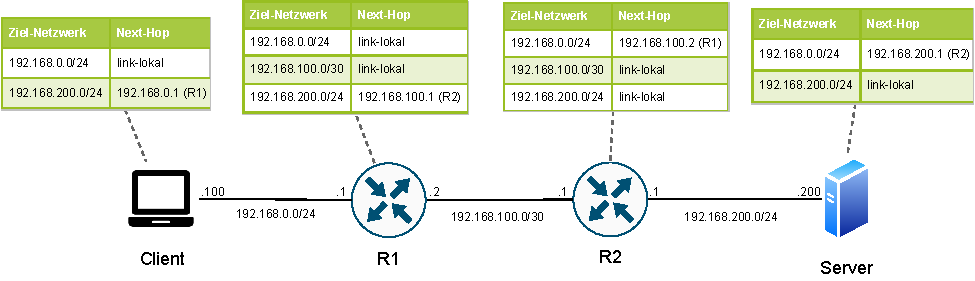
\includegraphics[scale=0.9]{Figures/next_hop_routing_specific_table.pdf}
  \caption{Next Hop Routing}
  \label{grafik: next_hop_routing}
\end{figure}\FloatBarrier
%TC:endignore
Client und Server müssen im Übrigen das Netzwerk 192.168.100.0/30 \textbf{nicht} in ihrer Routing-Tabelle pflegen. Dieses Netzwerk hat ausschließlich eine Relevanz zur Übertragung von Daten zwischen R1 und R2: Man spricht auch von Transfernetzwerken.\\
Dieses Beispiel bringt ein Skalierungsproblem mit sich: Umso mehr Subnetze existieren, in denen Server zu erreichen sind, desto mehr Routen muss der Client in der Routing-Tabelle, u.U. manuell gepflegt, vorhalten. Das gleiche gilt für Server, insofern eine Server-zu-Server-Kommunikation erfolgen soll.\\
In der Praxis sieht man kaum noch Endsysteme (darunter fallen Client und Server), welche mit solchen \textit{spezifischen} Routen arbeiten. Man überlässt die komplexe Verwaltung von Routing-Tabellen den Routern, während die Endsysteme neben der link-lokalen nur noch die \textit{Default}-Route besitzen. In diese Route 0.0.0.0/0 fallen alle Zielnetzwerke, abgesehen vom link-lokalen Subnetz, und sie zeigt immer auf den lokal erreichbaren Router.\\
Das Setzen der Default Route garantiert allerdings nicht, dass ein Ziel auch wirklich erreicht werden kann, z.B. weil es gar nicht existiert oder das Zielnetzwerk nicht in der Routing-Tabelle eines (Next-Hop-)Routers vorhanden ist. Ein Hilfsprotokoll zur Signalisierung von Erreichbarkeit ist dabei das Internet Control Message Protocol (ICMP). Das bekannte Werkzeug \texttt{ping} nutzt Nachrichten in Form von ICMP Echo Request und ICMP Echo Response, um die Erreichbarkeit via IP eines Endsystems zu prüfen.
\begin{figure}[h]
  \centering
  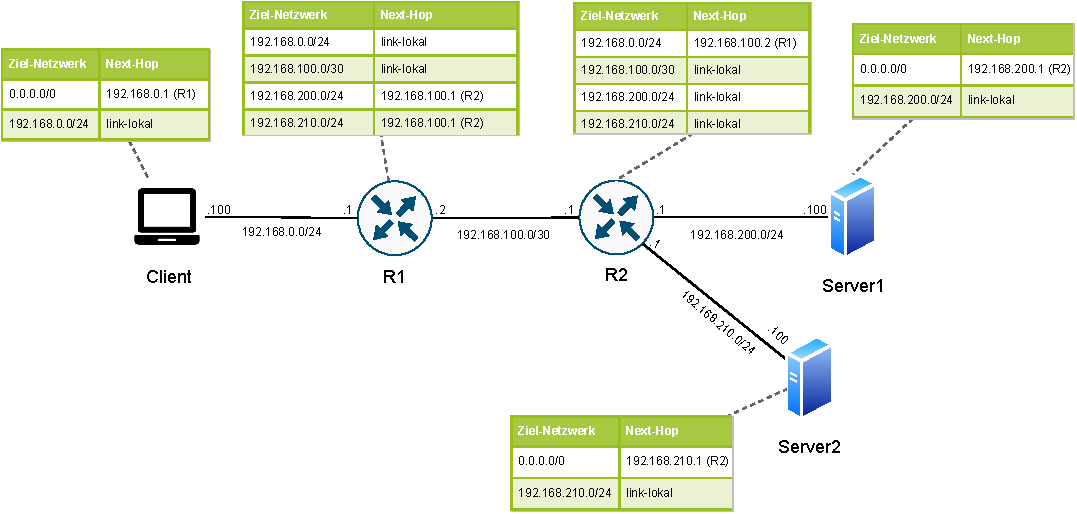
\includegraphics[scale=0.85]{Figures/next_hop_routing_default_route.pdf}
  \caption{Next Hop Routing mit Default Route}
  \label{grafik: next_hop_routing_with_default_route}
\end{figure}\FloatBarrier

Prinzipiell spielen im IPv4-Routing viele weitere Mechanismen eine zentrale Rolle: Zu nennen wären an dieser Stelle bspw. MAC-Adressen (Ethernet), Address Resolution Protocol (ARP), administrative Distanz und Time-To-Live (TTL). Für diese Ausarbeitung haben die Themen allerdings keine besondere Relevanz.\\

\textbf{\underline{Statisches IP-Routing}}\\
Bei nochmaliger Betrachtung der Abbildung \ref{grafik: next_hop_routing_with_default_route} erkennt man zwei Next-Hop Typen: link-lokal und \glqq IP-Adresse\grqq{}. Die link-lokale Route wird automatisch angelegt, sobald eine Netzwerkschnittstelle mit den entsprechenden Adressparametern konfiguriert wird.\\
Routen hingegen, die als Next-Hop eine IP-Adresse beinhalten, müssen entweder als statische oder dynamische Route den Weg in die Routing-Tabelle finden. Statische Routen sind Routen, bei denen ein Administrator Ziel-Netzwerk und Next-Hop manuell auf den Geräten pflegt.\\
Bis zu einer gewissen Netzwerkgröße lassen sich die Routing-Einträge statisch pflegen. Ab größeren Skalierungen mit vielen Routern und Zielnetzwerken wird die Administration jedoch problematisch. So kann es passieren, dass Router in der Konfiguration vergessen werden oder Routing-Einträge fehlen: dies macht eine Weiterleitung dann unmöglich und die Pakete werden verworfen.\\
Weiterhin bieten statische Routen wenig Flexibilität, wenn Verbindungen ausfallen: Es ist zwar möglich, Backup-Routen zu definieren, die zum gleichen Ziel über einen anderen Next-Hop führen mit Hilfe einer schlechteren \textit{Routing-Metrik}. Allerdings kann man nicht alle \textit{Fallback-Szenarien} des Routings vorab durchdenken.
%Routing Bild mit Dreieck

\textbf{\underline{Dynamisches IP-Routing}}\\
IP-Routing auf Basis von dynamischen Routing-Protokollen kann geschilderte Probleme umgehen, indem manuelle Administrationsaufwände verringert bzw. nicht erforderlich werden. Router, die ein dynamisches Routing-Protokoll nutzen, können gegenüber benachbarten Routern Erreichbarkeit für bestimmte Netzwerke signalisieren. Diese Information wird kaskadiert durch das gesamte Netzwerk getragen und es erhalten alle berechtigten Router einer \textit{Routing-Domäne} die Information, \textit{welche} Netzwerke erreichbar sind und \textit{wie} sie erreicht werden können. Auch Fallback-Szenarien sind durch dynamische Routing-Protokolle abgedeckt. Meist werden Backup-Routen schon im Speicher vorgehalten, um bei Ausfall einer Verbindung das Routing zu \textit{schwenken}. Man spricht auch von \textit{Routing-Konvergenz}.

\textbf{\underline{Border Gateway Protocol v4 (BGP)}}\\
Im Folgenden soll das Routing-Protokoll BGP betrachet werden. Dieses ist durch die Public Cloud-Provider vorgegeben, wenn dynamisches Routing gewünscht ist. Es ist ein so genanntes AS-Pfadvektorprotokoll. AS steht dabei für Autonomous System: Ein AS kann als eine administrative \glqq Grenze\grqq{} für eine Gruppe von Routern aufgefasst werden. Tauschen Router per BGP Routing-Informationen aus, spricht man auch von einem \textit{BGP-Peering}. Man unterscheidet an dieser Stelle zwischen internal BGP (iBGP) und external BGP (eBGP): Peerings innerhalb eines AS sind iBGP-Peerings, Peerings über AS-Grenzen hinweg sind eBGP-Peerings. iBGP dient dem Zweck, per eBGP gelernte Routen (\textit{(BGP-)Präfixe}) innerhalb eines AS weiterzutragen.

\begin{figure}[h]
  \centering
  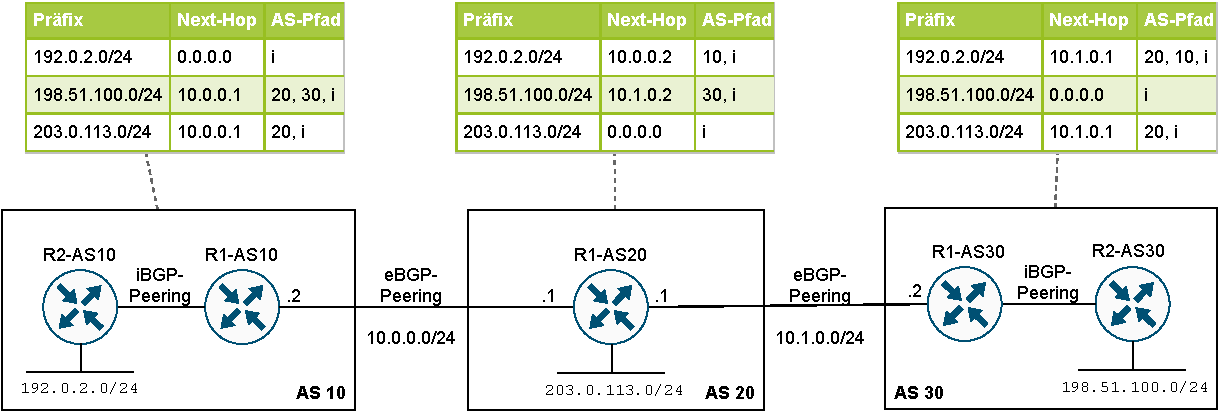
\includegraphics[scale=0.75]{Figures/ebgp_peerings.pdf}
  \caption{Verschiedene AS signalisieren Erreichbarkeit für Präfixe}
  \label{grafik: ebgp_peerings}
\end{figure}\FloatBarrier

Wie man auf der Abbildung \ref{grafik: ebgp_peerings} erkennt, werden drei Präfixe aus drei verschiedenen AS bekannt gemacht. Der AS-Pfad zeigt an, über welche AS ein Präfix erreicht werden kann. \textit{i} steht dabei für internal und stellt den Ursprung des Präfixes dar. Der Pfad wird von rechts (Ursprung) nach links gelesen.\cite{odom2010}\\
\textit{Anmerkung}: R2-AS10 kann mit dem Next-Hop 10.0.0.1 aus der Tabelle nichts anfangen: Dieser ist nur für R1-AS10 erreichbar. Im iBGP nutzt man daher das Attribut \textit{Next-Hop-Self}, womit iBGP-Nachbarn signalisiert wird, dass Next-Hop-Erreichbarkeit für ein Präfix \textit{über einen selbst} gegeben ist.\cite[S.468-471]{odom2010}\\
Die Next-Hop IP für Präfixe anderer AS zeigt bei R2-AS10 somit auf die IP von R1-AS10.

\begin{figure}[h]
  \centering
  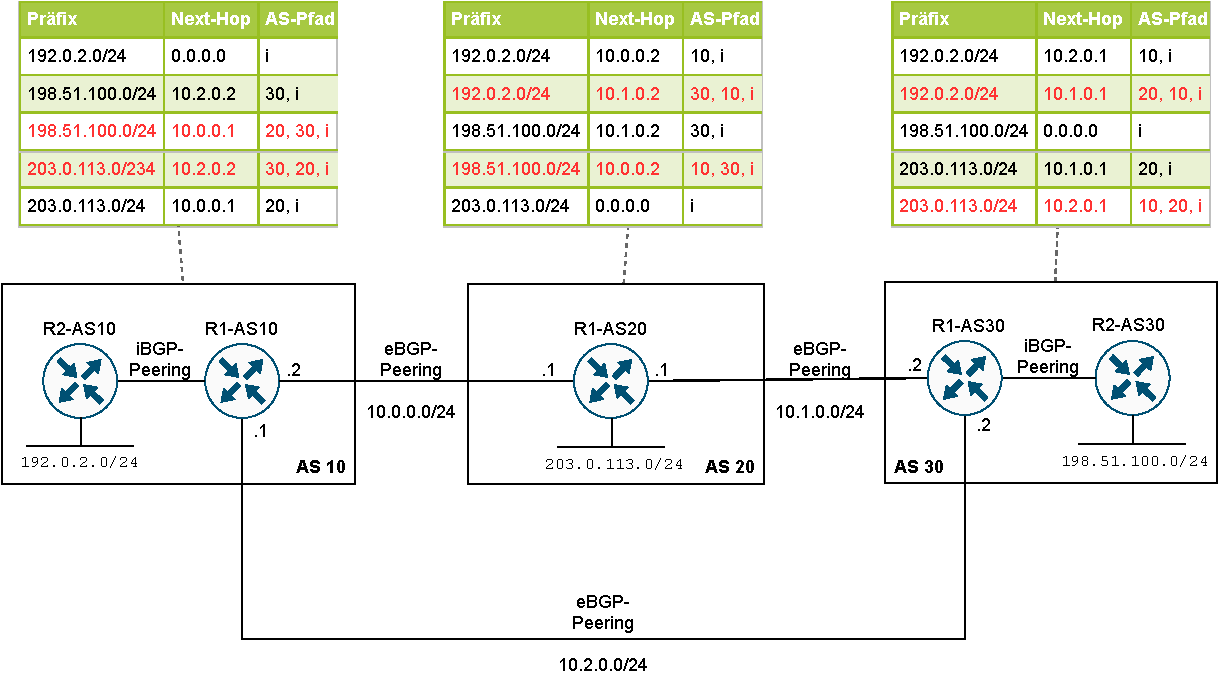
\includegraphics[scale=0.75]{Figures/ebgp_peerings_additional_connection.pdf}
  \caption{Gleicher Grundaufbau mit zusätzlicher Verbindung}
  \label{grafik: ebgp_peerings_additional_connection}
\end{figure}\FloatBarrier

In Listing \ref{grafik: ebgp_peerings_additional_connection} wurde noch eine Verbindung zwischen AS 10 und AS 30 hinzugefügt. Damit werden alle Präfixe, bis auf die eigenen, doppelt sichtbar, da sie nun über verschiedene Pfade erreicht werden können. Im Standardfall wird das Präfix mit dem kürzeren AS-Pfad bevorzugt.\\
Die Präfixe mit roter Schrift sind dabei allerdings nicht wertlos. Sie können als Backup-Pfad dienen, falls der bessere Pfad wegfallen sollte. Falls bspw. die Verbindung zwischen AS 10 und AS 30 ausfällt, \textit{konvergiert} das BGP auf allen Routern wieder hin zum Beispiel aus Abbildung \ref{grafik: ebgp_peerings}.\\
BGP-Router ignorieren AS-Pfade, in denen die eigene AS-Nummer bereits vorkommt. Pakete werden dann gemäß RFC 4271 verworfen. Dadurch werden effektiv Routing-Schleifen verhindert\cite{rfc4271}.\\
BGP sieht analog zu RFC 1918-Adressen Bereiche für AS-Nummern vor, die privat, also nicht im Internet, verwendet werden dürfen. Diese Nummern sind in RFC 6996 gelistet und gehen von einschließlich 64512 bis 65534\cite{rfc6996}.

%Cisco Doku
%next-hop self?
%BGP hat noch weitere \textit{Tie-Breaker}...
%AS-Pfad dient auch der Schleifenverhinderung
%64512–65534
%Beispieldiagramm


%Typische IGPs sind: OSPF, EIGRP, RIP, IS-IS
%Heutzutage findet nur noch ein EGP Verwendung: BGP

%Transfernetzwerk
%keine Metrik / AD
%Next Hops in Cloud funktionieren anders...
%In den Ursprüngen des Internets waren IP-Adressen \textit{classful}: die Netzwerkgröße wurde über die Klassenzugehörigkeit einer IP-Adresse bestimmt. Ein Class A Netz fiel in die \textit{Range} 0.0.0.0 - 127.255.255.255. So hätte obige IP-Adresse zu dem Class-A-Netzwerk "1.0.0.0" gehört

\subsection{Network Address Translation (NAT)}
Grundlegend geht es bei NAT darum, eine IP-Adresse \textit{umzuschreiben}. Dies ist sowohl für die Absender- als auch die Ziel-Adresse möglich. Dies kann verschiedene Gründe haben, oftmals geht es aber darum, IPv4-Adressen einzusparen.\\
Dies ist dem Umstand geschuldet, dass IPv4 nur einen Adressraum von 32 Bit hat, was $2^{32} \approx 4*10^9$ Adressen entspricht. Wenn man dagegen hält, dass die Weltbevölkerung zum Zeitpunkt der Arbeit knapp $8*10^9$ Menschen beträgt und viele Menschen bereits mehr als ein Endgerät besitzen, reicht der Adressraum bei weitem nicht mehr aus \cite{weltbevoelkerung2020dsw}.\\
Langfristig soll IPv6 mit einem Adressraum aus $2^{128}$ Bit IPv4 ablösen, doch selbst im Jahr 2021 fehlt weiterhin die \textbf{vollständige Unterstützung} einiger Hersteller für IPv6. Dies gilt ebenso für Public Cloud-Plattformen.\\
Der häufigste NAT-Mechanismus ist Network Address Port Translation (NAPT). Dabei können $n$ Clients hinter einer einzigen IPv4-Adresse \glqq verborgen\grqq{} und so IP-Adressen eingespart werden. Dafür werden neben der IP-Adresse bspw. noch Information der Transport-Schicht (Layer 4) wie Ports herangezogen, um NAPT-Sessions zuordnen zu können. Ein Router verwaltet diese Sessions in Form einer NAPT-Tabelle. Diese wird notwendig, wenn Rückpakete die verborgenen Clients erreichen sollen.\\
In dieser Ausarbeitung ist, wenn von NAT oder NATting gesprochen wird und keine anderweitigen Aussagen getroffen werden, der NAPT-Mechanismus gemeint.\\
Im Beispiel von Abbildung \ref{grafik: napt} werden drei Clients hinter einem Router geNATtet. Alle eingehenden Pakete werden auf die Quell-IP 10.1.0.1 umgeschrieben und es wird ein neuer Quell-Port vergeben. Wenn nun eine Verbindung von einem Client initiiert wird, sieht der Webserver lediglich die Quell-IP und den Quell-Port des Routers, welche durch das NAT vergeben wurden.\\
Rückpakete vom Webserver zu einem Client werden folgerichtig an den Router adressiert, welcher wiederum in der NAT-Tabelle nachschaut und die Pakete an den Client weiterleitet. Dafür müssen die Pakete auf das ursprüngliche Tupel aus Quell-IP und Quell-Port zurückgeschrieben werden.\\

\begin{figure}[h]
  \centering
  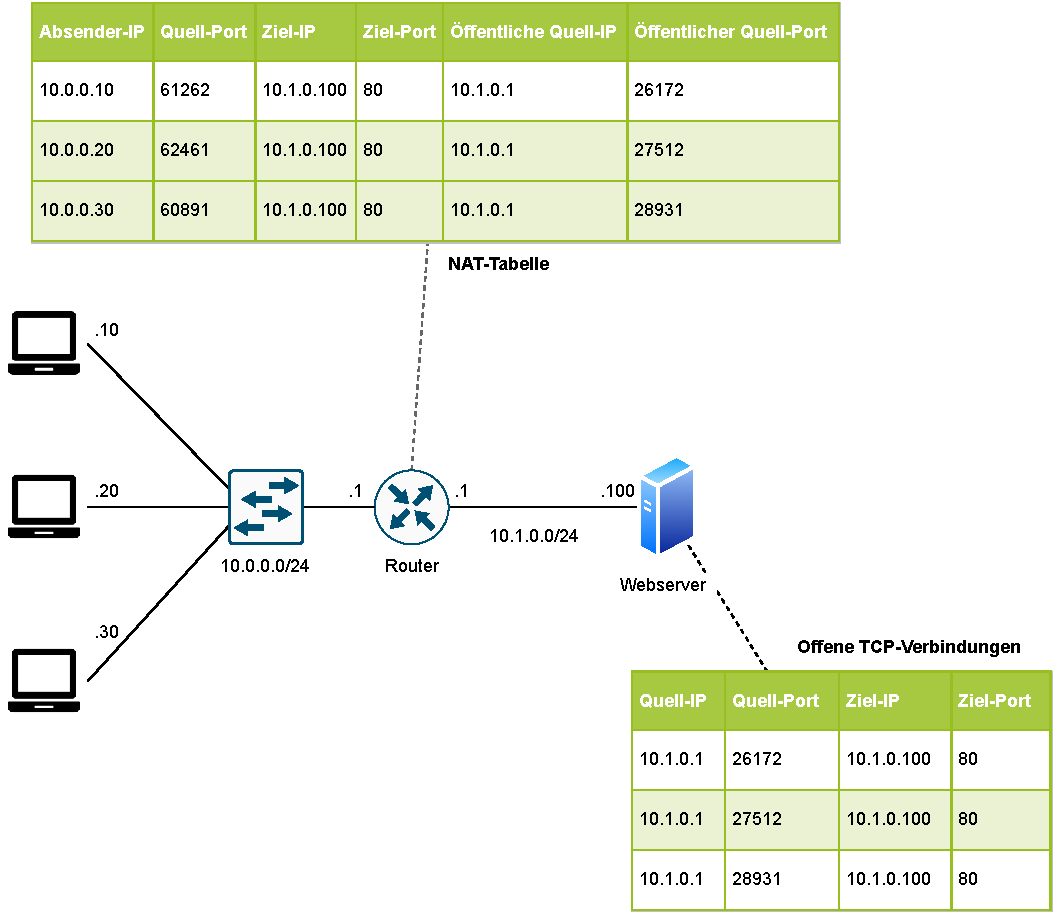
\includegraphics[scale=0.90]{Figures/napt.pdf}
  \caption{Beispiel Network Address Translation}
  \label{grafik: napt}
\end{figure}\FloatBarrier

NAT\label{nat-bad} verletzt das Prinzip der Ende-zu-Ende-Konnektivität: Findet sich für ein \textbf{vom Webserver kommendes} Paket in der NAT-Tabelle kein Eintrag, wird das Paket verworfen. Dies ist bei einer Client-zu-Server-Kommunikation oftmals kein Problem, da Verbindungen ohnehin vom Client initiiert werden und sich daraufhin ein State in der NAT-Tabelle des Routers befindet.\\
Wenn allerdings eine Client-zu-Client-Kommunikation stattfinden soll, ist man auf aufwändige Mechanismen wie z.B. Hole Punching angewiesen \cite[S.317]{Fall2011}.\\
Auf NAT soll daher in dieser Arbeit verzichtet werden, wenn dies möglich ist und es soll eine vollwertige Ende-zu-Ende-Konnektivität gewährleistet werden.

\subsection{Maximum Transmission Unit / Maximum Segment Size}\label{mtumss}
Die maximale Paketgröße auf einem Netzwerkmedium wird durch die Maxmimum Transmission Unit (MTU) beschrieben. Im Ethernet ist die \textit{Default}-MTU 1500 Byte.\cite[S.86]{Fall2011} Ethernet ist im Internet inzwischen das meistgenutzte Medium, daher haben sich auch hier diese 1500 Byte manifestiert.\\
Da die MTU auf dem Weg vom Empfänger zum Ziel variieren und auch mal geringer als 1500 Byte ausfallen kann, kann ein IPv4-Paket \textit{fragmentiert} werden. Dieser Prozess fordert Rechenzeit für Aufteilung und (Wieder-)Zusammensetzung in Fragmente und kann sich negativ auf die Performance (Latenz und Datendurchsatz) auswirken.\\
Man nutzt optimalerweise Path MTU Discovery oder beeinflusst die Maximum Segment Size für TCP (\glqq MSS-Clamping\grqq{}) bei Initiierung der Verbindung, um Fragmentierung (bestmöglich) zu umgehen.

\subsection{GeoIP}
Mit Hilfe von GeoIP-Datenbanken ist es möglich, den (ungefähren) Standort anhand der Absender-IP-Adresse eines Clients zu bestimmen. Verwendung finden solche Datenbanken häufig bei Internet-Streaming-Anbietern, um Zugriffe auf ein Videoangebot aus dem Ausland zu verhindern. Die Firma MaxMind ist dabei führender Anbieter für solche GeoIP-Datenbanken \cite{maxmind2021geoip}.

\section{Domain Name System (DNS)}\label{DNS}
Das DNS ermöglicht, Server im Internet anhand eines Namens, dem Fully Qualified Domain Name (FQDN), zu erreichen. Somit muss sich ein Benutzer einer Webseite keine IP-Adresse merken, sondern lediglich den dazugehörigen FQDN. Die IP-Adresse wird über die \textit{DNS-Auflösung} herausgefunden. Das DNS ist ein hierarchisches Modell, welches mit Domains arbeitet. Diese unterliegen unterschiedlichen Autoritäten. 
\begin{figure}[h]
  \centering
  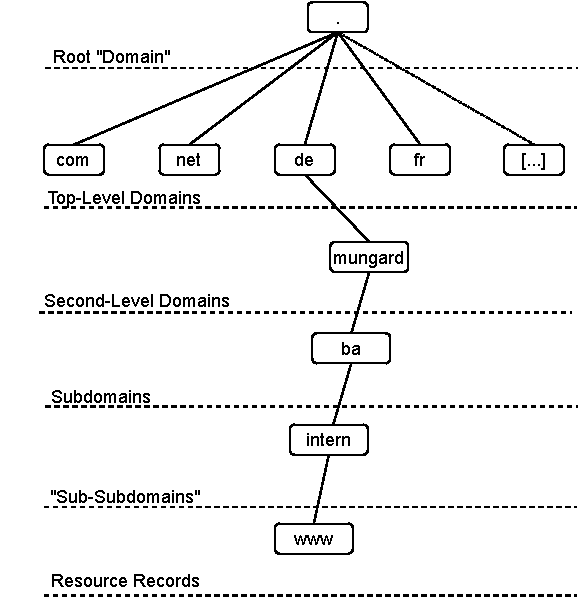
\includegraphics{Figures/dns_autoritative.pdf}
  \caption{DNS-Hierarchie}
  \label{grafik: dns-hierarchy}
\end{figure}\FloatBarrier

Soll z.B. der FQDN www.intern.ba.mungard.de. aufgelöst werden, muss der \textit{Baum} von der Wurzel \glqq .\grqq{} über die Knoten \glqq de\grqq{}, \glqq mungard\grqq{}, ... bis zum Blatt \glqq www\grqq{} durchlaufen werden. Man spricht von einer iterativen Auflösung. Pro Hierarchie-Ebene sind \textit{autoritative Nameserver} verantwortlich für die richtige Delegation des auflösenden Clients.\\
Das Blatt \glqq www\grqq{} wird auch als Resource Record bezeichnet. Für diese Arbeit sind lediglich A-Records relevant, welche FQDN nach IPv4-Adresse auflösen. Viele weitere DNS-Records existieren, z.B. für IPv6-Adressen (AAAA) oder um Mailserver (MX) für eine Domain anzugeben \cite[S.528]{Fall2011}. Ein Beispiel für einen autoritativen Nameserver ist Bind \cite{liu2006dns}. Innerhalb des Nameservers werden Domains anhand von \textit{Zonen(-Dateien)} verwaltet.

\subsection{DNS-Resolver}
Endgeräte machen diese iterative Namensauflösung typischerweise nicht selbst, sondern leiten ihre Anfragen an einen DNS-Resolver weiter (\textit{Forwarding}). Dieser ist in Abbildung \ref{grafik: dns-resolver} dafür verantwortlich, zu einem FQDN eine IPv4-Adresse zu finden (iterativ) und dem Endgerät zurückzuliefern. Wenn ein Nameserver für eine gesuchte Domain nicht autoritativ, ist wird der DNS \textit{Client} (hier der Resolver) per NS Record weiterdelegiert.

\begin{figure}[h]
  \centering
  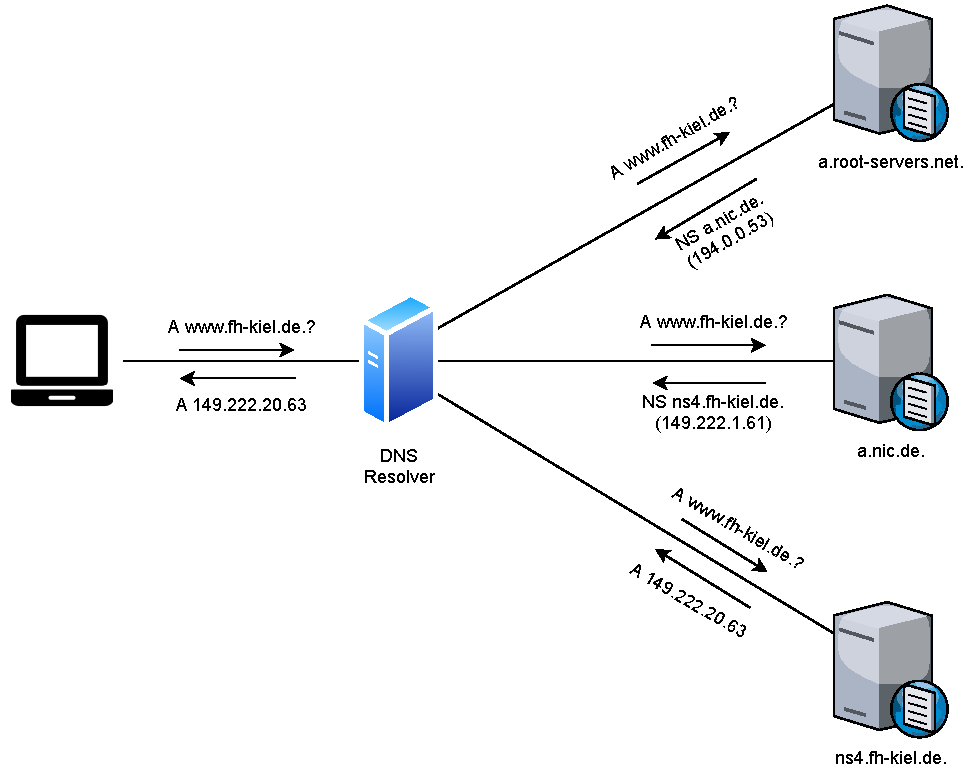
\includegraphics{Figures/dns_recursion.pdf}
  \caption{DNS-Resolver}
  \label{grafik: dns-resolver}
\end{figure}\FloatBarrier
%TC:ignore
\begin{listing}[h]
\begin{minted}[breaklines,frame=single]{bash}
$ dig www01.fh-kiel.de @8.8.8.8 | grep -v '^$'
; <<>> DiG 9.11.9 <<>> www01.fh-kiel.de @8.8.8.8
;; global options: +cmd
;; Got answer:
;; ->>HEADER<<- opcode: QUERY, status: NOERROR, id: 11777
;; flags: qr rd ra ad; QUERY: 1, ANSWER: 1, AUTHORITY: 0, ADDITIONAL: 1
;; OPT PSEUDOSECTION:
; EDNS: version: 0, flags:; udp: 512
;; QUESTION SECTION:
;www01.fh-kiel.de.              IN      A
;; ANSWER SECTION:
www01.fh-kiel.de.       21599   IN      A       149.222.20.63
;; Query time: 60 msec
;; SERVER: 8.8.8.8#53(8.8.8.8)
;; WHEN: Tue May 18 22:21:45 CEST 2021
;; MSG SIZE  rcvd: 61
\end{minted}
\label{dig-example-fh-kiel}
\caption{Eine DNS-Auflösung für einen A-Record (www01.fh-kiel.de) gegen den Resolver von Google (8.8.8.8)}
\end{listing}\FloatBarrier
%TC:endignore


Weiterhin kann ein Resolver Einträge \textit{cachen}, um auf erneute Anfragen für gleiche FQDN schneller zu antworten.%Der letzte Punkt eines FQDN, welcher die Root-Domain repräsentiert, wird üblicherweise ausgelassen.

\subsection{Split DNS}
Split DNS ist die Möglichkeit, verschiedene Resource Records anhand der Absender-IP auszuliefern. Dafür pflegen autoritative Nameserver Access Control Lists (ACL) mit verschiedenen IP-Präfixen, um eine Fallunterscheidung treffen zu können\cite[S.565-567]{Fall2011}. Dies ist z.B. relevant, wenn eine Firma zwischen internen und externen Anfragen unterscheiden muss, um den (richtigen) Zugriff auf Ressourcen zu gewährleisten.

\begin{figure}[h]
  \centering
  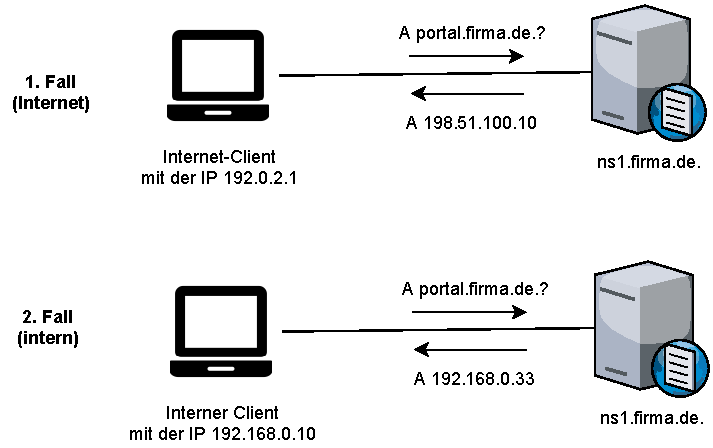
\includegraphics{Figures/dns_split_view.pdf}
  \caption{Split DNS für portal.firma.de.}
  \label{grafik: split-dns}
\end{figure}\FloatBarrier

\subsection{DNS UPDATE}
Die Methode DNS UPDATE ist in RFC 2136 definiert und erlaubt es, autoritative Zonen eines Nameserver zur Laufzeit zu verändern\cite{rfc2136}. Somit müssen keine Zonen-Dateien manuell angepasst werden. Außerdem muss der Nameserver nicht neugestartet werden, um die editierten Zonen-Dateien neu einzulesen.\\
Clients werden über eine ACL ermächtigt, diese Updates zu tätigen. Dabei kann die Absender-IP zur Authentifizierung genutzt werden: Allerdings ist diese Methode unsicher, da sich IPs \textit{spoofen} lassen. Sicherer ist es, mit Hilfe eines vorab ausgetauschten Schlüssels (\textit{Pre-Shared Key}) eine DNS UPDATE-Nachricht zu signieren. Dies passiert mit Hilfe von Transaction Signatures (TSIG) \cite[S.911-914]{Fall2011}.

\section{Virtual Private Network (VPN)}\label{vpn}
VPNs werden genutzt, um private Netzwerke über eine öffentlich genutzte Infrastruktur abbilden zu können. Dies erfolgt zwischen VPN-Endpunkten über gängige Enkapsulierungen, z.B. Generic Routing Encapsulation (GRE), Encapsulating Security Payload (ESP) oder OpenVPN.\\
In Abbildung \ref{grafik: vpn-example} werden Daten von Client A zu Client B über das Internet zwischen Router R1 und Router R2 enkapsuliert. R2 empfängt das Datenpaket, packt es aus und sendet es in der ursprünglichen Form weiter an Client B.\\
Das Diagramm ist dabei nicht spezifisch für eine bestimmte VPN-Technologie. Es können, je nach Technologie, Nutzdaten verschlüsselt werden. 
\begin{figure}[h]
  \centering
  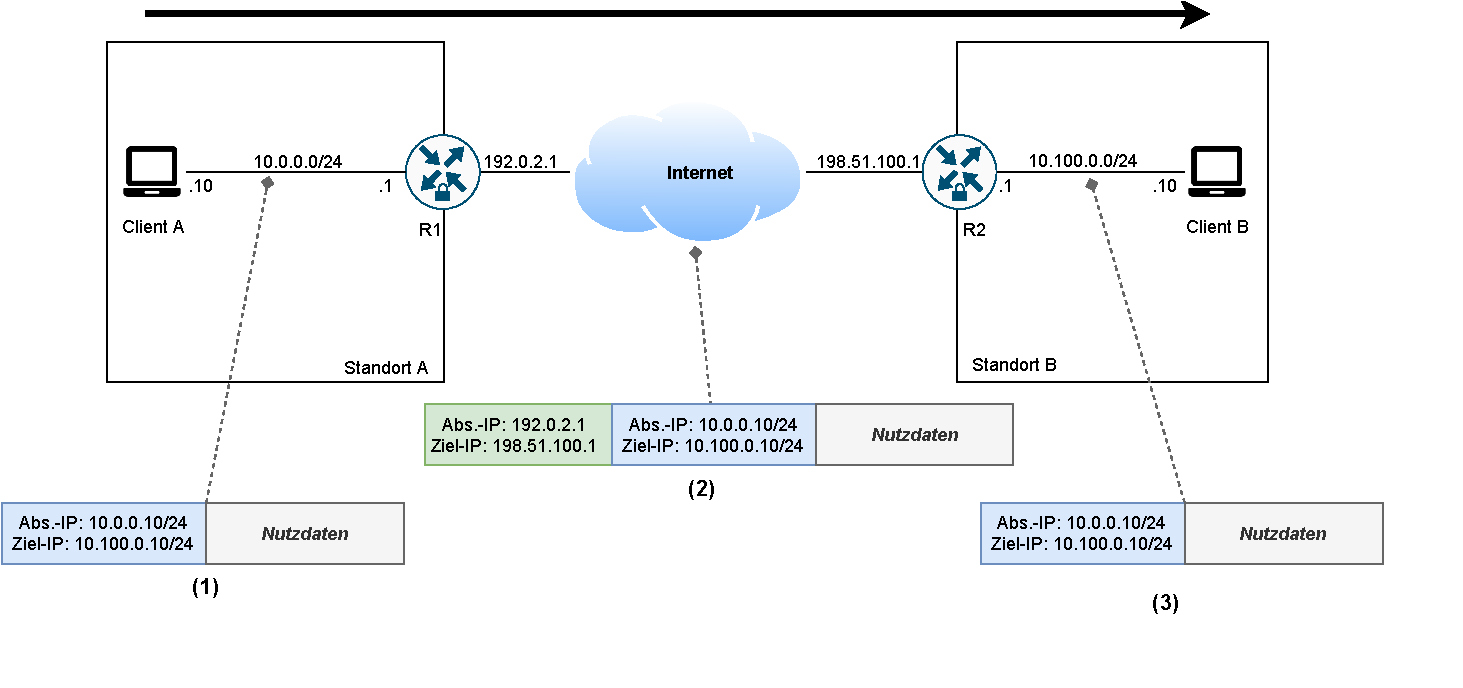
\includegraphics[scale=0.65]{Figures/vpn-example.pdf}
  \caption{Übertragung eines IP-Pakets über einen VPN-Tunnel}
  \label{grafik: vpn-example}
\end{figure}\FloatBarrier

%Quelle
Die in dieser Arbeit verwendeten VPN-Technologien sind IPsec und OpenVPN. IPsec wird u.a. für die Vernetzung von (Cloud-)Standorten, auch Site-to-Site (S2S) genannt, genutzt und arbeitet auf OSI-Schicht 3. Ebenso dient es zur \textit{Einwahl} in (Firmen-)Netzwerke. IPsec wird meist im Geschäftsumfeld genutzt und es exisitieren viele herstellerabhängige Implementationen.\\
OpenVPN ist ein Open Source-Projekt und es nutzt \textit{Transport Layer Security} (TLS) für die verschlüsselte Übertragung von Daten via UDP oder TCP. Das Protokoll ist auf OSI-Schicht 7 zu finden und es wird vor allem für Client-to-Site-Verbindungen genutzt (C2S): Passende Software ist für viele verschiedene Plattformen verfügbar (u.a. Windows, Linux, Mac, Android) und sowohl Client- als auch Server-Applikation sind kostenfrei erhältlich.\\
Angesprochene MTU-Probleme (s. \ref{mtumss}) können sich bei einer getunnelten Verbindung auf Grund des zusätzliches \textit{Overheads} auf Grund der Enkapsulierung zeigen. Eine IP-Fragmentierung sollte optimalerweise verhindert werden.

\section{Cloud}\label{cloud}
%VyOS PaaS? VyOS kann als hybrid zwischen IaaS und PaaS angesehen werden, da man die virtuelle Maschine bis auf CPU nichts weiter konfigurieren kann... und sie ist für Infrastruktur verantwortlich...
Der Cloud-Begriff kann je nach Literatur variieren. Diese Arbeit verweist an dieser Stelle auf die Definition des \textit{National Institute of Standards and Technology (NIST)}. Ebenso werden dort die drei typischen \textit{Cloud Delivery}-Modelle Software as a Service (SaaS), Platform as a Service (PaaS) und Infrastructure as a Service (IaaS) definiert, welche fortan als bekannt vorausgesetzt werden.\cite{mell2011}

\subsection{Public und Private Cloud}
Auch für die so genannten \textit{Cloud \gls{Deployment}}-Modelle wird auf die Definition des NIST verwiesen.\cite{mell2011}\\
Allerdings soll an dieser Stelle ein häufiges Missverständnis hingewiesen werden: Eine Private Cloud existiert nicht zwingend \textit{on-premises} einer Organisation, also bspw. im eigenen Rechenzentrum. Sie kann ebenso über Public Cloud-Plattformen abgebildet werden. Allerdings ist die Voraussetzung, dass alle genutzten Ressourcen dann exklusiv für die Organisation zur Verfügung stehen (\textit{exclusive use by a single organization}). Sie werden nicht mit weiteren Parteien geteilt (\textit{open use by the general public}).\\
%Abgrenzung Private Cloud ...irgendwo... einarbeiten. Es wird angenommen, dass die Private Cloud schon besteht. Router interessiert, bißchen Infrastrukut (Webserver), Rest interessiert nicht...
Die Public Cloud-Provider, welche in dieser Arbeit genutzt werden, sind Amazon Web Services (AWS) und Microsoft Azure. Rechenzentren stehen weltweit zur Verfügung, um eine schnelle und latenzarme Anbindung für die Kunden zu ermöglichen. Eine Private Cloud lässt sich bspw. mit OpenStack abbilden\cite{sefraoui2012openstack}.

\subsection{Multi und Hybrid Cloud}
Eine Multi Cloud vernetzt \textbf{gleiche} Cloud \gls{Deployments} miteinander, z.B. Public Cloud 	$\leftrightarrow$ Public Cloud oder Private Cloud $\leftrightarrow$ Private Cloud.\\
Bei einer Hybrid Cloud werden unterschiedliche Bausteine zusammengefasst. In dieser Arbeit soll eine Hybrid Cloud aus AWS, Azure (Public) und Private Cloud bereitgestellt werden.

\section{Public Cloud-Netzwerke}\label{public-cloud-networking}
In diesem Kapitel wird näher auf die verschiedenen Netzwerk-\textit{Building Blocks} der Public Cloud-Plattformen AWS und Azure eingegangen. Beide bringen oftmals ähnliche Bausteine mit. Es wird daher stets versucht, im jeweiligen Kontext auf beide Plattformen zugleich einzugehen, um die Grundfunktionalität zu erläutern.
Dieses Kapitel vermittelt lediglich Grundlagen, die für das Verständnis der Use-Cases notwendig sind. Besonderheiten und Constraints, die sich im Verlauf der Bearbeitung ergeben haben, werden im jeweiligen Use-Case unter \glqq Probleme und Lösungsfindung\grqq{} zusammengefasst.

\subsection{AWS VPC / Azure VNET}
AWS Virtual Private Cloud (VPC) und Azure Virtual Network (VNET) bilden private Netzwerke innerhalb eines Cloud-Mandanten ab. Die hier hinterlegten Präfixe bilden eine Menge an möglichen IP-Adressen innerhalb von VPC und VNET ab. Es können sowohl Public IP-Präfixe als auch IPs nach RFC 1918 benutzt werden. Diese Menge an IP-Adressen wird in AWS \textit{CIDR} bzw. Azure \textit{Address Space} als Container zusammengefasst.\\
AWS gibt /16 als minimale und /28 als maximale Größe des CIDR vor \cite[S.100]{awsug2020}. Azure VNET ist da großzügiger und es darf eine Größe zwischen /8 und /29 gewählt werden\cite[S.10]{Toroman2019}. 
\subsection{Subnets}
Innerhalb von VPC und VNET können Subnets angelegt werden. In diesen Subnets können bspw. virtuelle Maschinen mit IPs ausgestattet werden. Wenn also ein VPC ein CIDR-Präfix von 10.0.0.0/16 besitzt, kann z.B. ein Subnet 10.0.1.0/24 \glqq herausgeschnitten\grqq{} werden. Mit Subnets können weitere Objekte verknüpft werden wie z.B. Route Tables, welche das Routing für das Subnet steuern.

\subsection{Route Tables}
Route Tables ermöglichen es, den Fluss von IP-Pakete innerhalb eines Subnets zu steuern. So können z.B. statische Routen auf Ziele innerhalb eines Subnets angelegt werden. VNET kann dies, wie aus dem klassischen Netzwerk gewohnt, über Next-Hop IPs abbilden. VPC hingegen unterstützt als Next-Hop virtuelle Maschinen (Instances) und Interfaces von virtuellen Maschinen. Es existieren noch weitere spezielle Ziele, die genutzt werden können wie z.B. VPN Gateways, um entfernte Netzwerke zu erreichen.\\
Subnets in Azure erfordern keine Route Tables: Alle Maschinen eines VNET erreichen sich untereinander standardmäßig und erreichen Ressourcen im Internet. Sollte ein granulareres Routing notwendig sein, werden Azure Route Tables erforderlich.\\
Subnets in VPC erhalten immer eine Route Table: Ohne weitere Konfigurationen wird einem Subnet die Main Route Table zugewiesen. Diese kann vorab editiert werden, so dass z.B. kein Internet-Traffic für virtuelle Maschinen möglich ist. \textit{Non-Main} Route Tables können für spezielle Anforderungen erstellt und Subnets zugewiesen werden.

\subsection{Security Groups}
AWS Security Groups (SG) bzw. Azure Network Security Groups (NSG) bilden \textit{stateful Firewalling} ab \cite{wool2006packet}. Dabei können sowohl ingress (eingehende), als auch egress (ausgehende) Firewall-Regeln definiert und darauf basierend Pakete gefiltert werden. Typische Protokolle anhand derer Regeln definiert werden können sind UDP, TCP und ICMP.\\
AWS SGs können einer Instanz zugewiesen werden. Wird keine SG explizit für eine Instanz definiert, kommt eine Default SG zu Einsatz, die vom VPC vorgegeben ist.\\
Azure NSGs können sowohl Subnets als auch VMs direkt zugewiesen werden. NSGs für Subnets wirken sich global für alle VMs eines Subnets aus. Wenn granularer Zugriff auf bestimmte VMs gewünscht ist, nutzt man zusätzliche NSGs \glqq auf\grqq{} den jeweiligen Instanzen.

\subsection{VPN}
AWS bringt in Form von Virtual Private Gateway und Transit Gateway Möglichkeiten mit, IPsec-basierte S2S-Verbindungen zu terminieren. Ersteres kann Verbindungen nur innerhalb eines VPC terminieren. Transit Gateway bietet die Möglichkeit, verschiedene VPCs miteinander zu \textit{peeren}. VPN-Verbindungen können auf Transit Gateway terminiert werden und Pakete, die über VPN reinkommen, können alle gepeerten VPCs erreichen.\\
Azure Virtual network gateway kann analog zu AWS Virtual Private Gateway IPsec-Tunnel in einem VNET terminieren.\\
AWS und Azure ermöglichen innerhalb der Tunnel die Nutzung von BGP, um dynamische Routing-Informationen miteinander auszutauschen.


\section{Automatisierung}\label{automatisierung}

Diverse Automatisierungswerkzeuge ermöglichen es, gewünschte Endzustände von Systemen zu definieren. Mit heutigen Werkzeugen wie z.B. \textit{Ansible} muss ein Administrator wenig Programmiererfahrungen mitbringen und schreibt die gewünschten Parameter in eine Konfigurationsdatei, die zu einem gewünschten Zeitpunkt auf Systemen ausgerollt werden. Viele Probleme wurden bereits von anderen Community-Mitgliedern gelöst. Für komplexere Sachverhalte existieren Plugins.\\
Man muss bei Automatisierungswerkzeugen zwischen \textit{Configuration Management} (CM) und \textit{Provisioning} unterscheiden. Provisioner dienen der grundsätzlichen Erstellung einer Infrastruktur, während CM-Werkzeuge diese Infrastruktur als vorhanden annehmen und weitere Konfigurationen auf den jeweiligen Komponenten tätigen\cite[S.20]{Brikman2019}.\\
Eine Analogie wäre: Provisioner setzen das Haus an eine Straße und das CM macht daraufhin die Innenaustattung. Auf die IT angewendet bedeutet dies, dass Provisioner dafür sorgen, dass Ubuntu-Maschinen aufgesetzt werden und zu erreichen sind. Das CM macht daraufhin Paket-Updates und installiert z.B. einen Apache-Webserver.\\
Es gibt keine klare Linie zwischen den beiden Typen von Werkzeugen. So können viele CM-Werkzeuge auch eine Provisionierung von Infrastruktur abbilden, während Provisioner auch grundlegendes Configuration Management leisten können\cite[S.20]{Brikman2019}. Das bereits angesprochene Ansible ist eher als CM-Tool zu sehen.\\
Passende Schnittstellen, z.B. in Form einer REST-API, sind Voraussetzung, um Automatisierungswerkzeuge mit entsprechenden Komponenten nutzen zu können.

\subsection{Terraform}
Das Werkzeug, das hauptsächlich für Automatisierungs-Schritte in dieser Arbeit verwendet wird, ist \textit{Terraform} der Firma Hashicorp. Es ist ein Provisioner mit begrenzten Möglichkeiten für Configuration Management. Es besitzt eine Vielzahl an \textit{Resources}, welche es ermöglichen, Infrastruktur-Komponenten reproduzierbar bereitzustellen. Es wird eine deklarativer Sprachstil genutzt, um gewünschte Zustände der Infrastruktur zu beschreiben. Man spricht auch von \textit{Infrastructure as Code} (IaC).

\textbf{\underline{Provider}}\\
Provider sind die Grundvoraussetzung, um die Automatisierung einer Plattform mit Terraform bewerkstelligen zu können. Sie ermöglichen es, mit entsprechenden Schnittstellen der Anbieter, z.B. REST, zu interagieren. Provider liefern meist diverse \textit{Resources} mit, welche Veränderungen tätigen können und \textit{Data Sources}, welche \glqq lesend\grqq{} auf die Infrastruktur zugreifen, um Informationen zurückzuliefern. Diese Informationen können dann anderen \textit{Modulen} zur Verfügung gestellt werden.\cite{Brikman2019}\\
%Serifen-Schrift für Dateinamen...
Terraform arbeitet stateful: Nach jedem \texttt{terraform apply}, welches zur Erstellung der gewünschten Infrastruktur führt, werden Referenzen aller Infrastrukturkomponenten in der Datei \underline{terraform.tfstate} gespeichert: Ein erneuter Aufruf von \texttt{terraform apply} würde, insofern keine Konfigurationsänderungen gemacht wurden, die Infrastruktur so belassen und sie nicht nochmals bereitstellen bzw. erweitern. Per \texttt{terraform destroy} kann die Infrastruktur wieder zurückgebaut werden.\\
In Listing \ref{tf-aws-provider-example} wird der Provider \textit{aws} in einer spezifischen Version eingebunden. Der Constraint \glqq $\sim$>\grqq{} sorgt dafür, dass nur Versionen des Providers innerhalb des 3.35.x Branches benutzt werden (\glqq Minor Patches\grqq{}).
%TC:ignore
\begin{listing}[h]
\begin{minted}[breaklines,frame=single]{tf}
terraform {
    required_providers {
        aws = {
            source = "hashicorp/aws"
            version = "~> 3.35.0"
        }
    }
}
\end{minted}
\caption{Terraform AWS Provider}
\label{tf-aws-provider-example}
\end{listing}
%TC:endignore
\textbf{\underline{Resources}}\\
Resources erstellen Infrastuktur-Komponenten und statten diese mit den richtigen Parametern aus. In \ref{deployment_aws_tf} wird ein VPC mit dem CIDR-Block 10.0.0.0/16 und ein darunterliegendes Subnet 10.0.1.0/24 erstellt.
%TC:ignore
\begin{listing}[h]
\begin{minted}[breaklines,frame=single]{tf}
resource "aws_subnet" "example_subnet" {
    vpc_id            = aws_vpc.example_vpc.id
    cidr_block        = "10.0.1.0/24"
    availability_zone = "eu-central-1"
}
resource "aws_vpc" "example_vpc" {
    cidr_block = "10.0.0.0/16"
}
\end{minted}
\caption{Deployment der Resources \glqq example\_vpc\grqq{} und \glqq example\_subnet\grqq{}}
\label{deployment_aws_tf}
\end{listing}
%TC:endignore
Dabei zeigt sich auch der deklarative Aspekt von Terraform. Die Resource \glqq aws\_subnet\grqq{} mit dem Namen \glqq example\_subnet\grqq{} kommt als erstes im Code vor, referenziert jedoch das VPC \glqq example\_vpc\grqq{}. Durch diese impliziete Abhängigkeit wird die Resource \glqq example\_vpc\grqq{} als erstes erstellt. Man beschreibt also, \textit{was} benötigt wird. \textit{Wie} und in welcher Reihenfolge das Rollout gemacht wird, obliegt Terraform.

\textbf{\underline{Module}}\\
Terraform Module sind \textit{Container}, die mehrere Resources in *.tf-Dateien zusammenfassen \cite{tfmodule2021}. Es ist zwar möglich, alle notwendigen Resources in einer einzigen *.tf-Datei zu konfigurieren, allerdings ist es \textit{best practice}, verschiedene Resources der Übersichtlichkeit wegen aufzuteilen und in einer geeigneten Ordnerstruktur unterzubringen. Die jeweiligen Dateien innerhalb eines Ordners heißen dann \underline{main.tf}. Um Attribute an andere Module weiterzugeben, werden \textit{Outputs} genutzt. 

\textbf{\underline{Data Sources und Outputs}}\\
Data Sources führen keine Änderung herbei, sondern werden genutzt, um detaillierte Informationen zu Infrastruktur-Komponenten zurückzugeben oder um etwas zu finden. In Listing \ref{data-source-find-output-id} wird nach einem Amazon Machine Image (AMI) für Ubuntu gesucht. Die ID (image\_id) für das \textit{most recent} Release kann per Output an andere Module weitergegeben werden. Diese können die ID dann z.B. nutzen, um per Resource eine virtuelle Maschine mit dem gewünschten Ubuntu-Image bereitzustellen.
%TC:ignore
\begin{listing}[h]
\begin{minted}[breaklines,frame=single]{tf}
data "aws_ami" "ubuntu" {
  most_recent = true
  filter {
    name   = "name"
    values = ["ubuntu/images/hvm-ssd/ubuntu-focal-20.04-amd64-server-*"]
  }
  filter {
    name   = "virtualization-type"
    values = ["hvm"]
  }
  owners = ["099720109477"] # Canonical
}
output "ubuntu_ami_id" {
  value = data.aws_ami.ubuntu.image_id
}
\end{minted}
\caption{Die Data Source \glqq ubuntu\grqq{} sucht nach dem passenden Ubuntu Image und Output macht die ID global für andere Module verfügbar}
\label{data-source-find-output-id}
\end{listing}
%TC:endignore
\subsection{IP Address Management (IPAM)}
Ein IPAM ist wichtig, insofern die Adressverwaltung automatisiert werden soll. Statisch konfigurierte CIDR-Blöcke im Code sorgen für eine schlechte Wiederverwendbarkeit und Skalierbarkeit von Modulen: IP-Blöcke müssten dann jedes Mal händisch reserviert und in den gewünschten Modulen untergebracht werden.\\
Einfacher ist es, im Modul lediglich festzulegen, welche Subnetzgröße erforderlich ist: ein IPAM gibt dann den nächsten freien Block in der passenden Größe zurück. Es wird lediglich ein großer Block vorreserviert, aus dem die freien Blöcke entnommen werden können.

\begin{figure}[h]
  \centering
  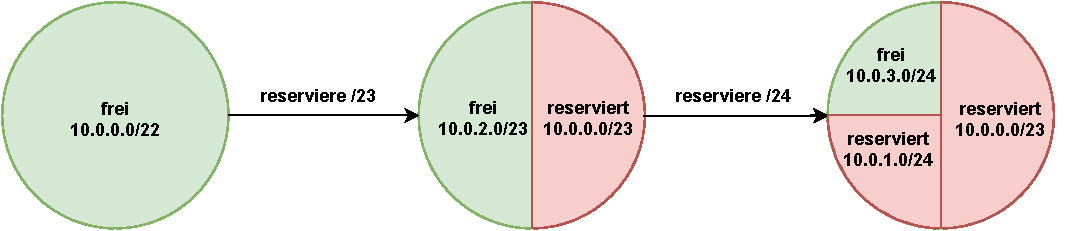
\includegraphics[scale=0.8]{Figures/ipam_cake.pdf}
  \caption{IPAM-Reservierung von CIDR-Blöcken}
  \label{grafik: ipam_ip_reservation}
\end{figure}\FloatBarrier
